\documentclass[12pt,a4paper]{article}
\synctex=1
\usepackage[utf8]{inputenc}
\usepackage[margin=1cm]{geometry}
\usepackage{graphicx}
%\usepackage{verbatim}
\usepackage{listings}
\usepackage{textcomp}
\usepackage{courier}
\usepackage{libertine}
\usepackage{pgfornament}
\usepackage{eso-pic}
\usepackage[hangul]{kotex}
\linespread{1.3}

\title{
	\centering
	\pgfornament[width=12cm,color=teal]{84}\\
	\vspace{1cm}
	\fontsize{50}{50} \selectfont {컴퓨터 그래픽스 입문}\\
		\pgfornament[width=12cm,color=teal]{88}\\
	\vfill}
\author{
	\LARGE
	\begin{tabular}{rl}
		\hline
		학번 : & 2016110056\\ 
		학과 : & 불교학부 \\
		이름 : & 박승원\\
		날짜 : & \today\\
		\hline
	\end{tabular}\vspace{2cm}
	\\

\includegraphics[width=0.5\textwidth]{logo.jpg}
	}
\date{}


\begin{document}
\maketitle
\pagenumbering{gobble}
\noindent
\lstset{language=C++, columns=flexible, tabsize=4, frame=shadowbox, showstringspaces=false, breaklines=true, upquote=true, basicstyle=\normalsize}

\section{Shader Programming}
1. Send color array to your vertex shader to draw a color box as you did last week. (5pt)

2. Use uniform matrix 4x4 to rotate your box in vertex shader.(5pt)

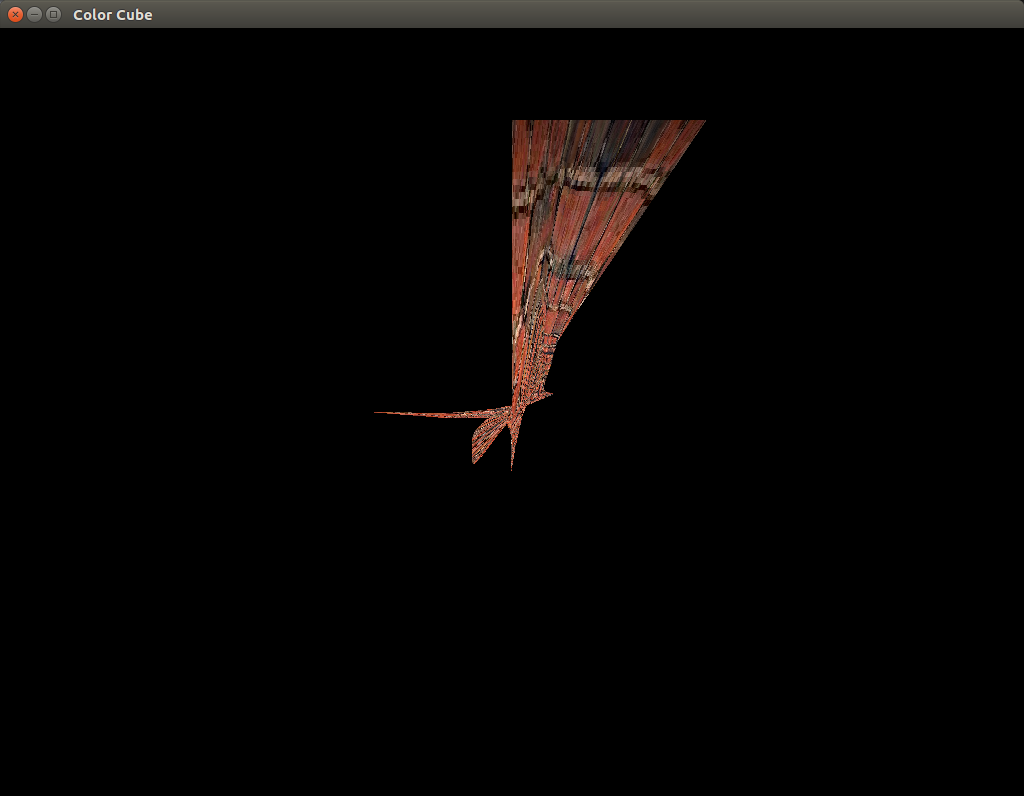
\includegraphics[width=\textwidth]{1.png}

\lstinputlisting[caption=vertex shader]{src/vertex_shader.glsl}	
\lstinputlisting[caption=fragment shader]{src/fragment_shader.glsl}	
\lstinputlisting[caption=메인함수]{src/val.cpp}	

shader 프로그램을 만들고 변수를 보내는 make shader program 이란 함수를 만들었다.\\
또, 매트릭스 데이터를 보내고 바인드하는 transfer matrix 함수도 만들었다.\\
내가 만든 매트릭스는 자료구조가 약간 달라 transpose 한 후에 데이터를 보내야 되었다.\\
밑의 callbacks.cc의 하단에 있으니 참조바랍니다.\\

프로그램은 이전에 만들어두었던 큐브를 그대로 사용하여, 데이터를 세이더에 보내고, 바인드하는 작업을 한다.\\
세이더에서 입력받을 변수를 선언하고, vbo를 배열로 일렬로 만든 후, 바인드하면 되었다.
\lstinputlisting[caption=callbacks.cc]{src/callbacks.cc}
	
\end{document}
